%\documentclass[letterpaper, 10 pt, conference]{ieeeconf}

\documentclass[a4paper, 10pt, conference]{ieeeconf}      
\IEEEoverridecommandlockouts                                                                                  
\overrideIEEEmargins
\usepackage[utf8]{inputenc}
\usepackage{graphicx}
\usepackage{kotex}
\usepackage{amsmath}
\usepackage{graphicx}
\usepackage{geometry}
\usepackage{cite}
\usepackage{cleveref}
\usepackage[T1]{fontenc}

% The following packages can be found on http:\\www.ctan.org
%\usepackage{graphics} % for pdf, bitmapped graphics files
%\usepackage{epsfig} % for postscript graphics files
%\usepackage{mathptmx} % assumes new font selection scheme installed
%\usepackage{mathptmx} % assumes new font selection scheme installed
%\usepackage{amsmath} % assumes amsmath package installed
%\usepackage{amssymb}  % assumes amsmath package installed

\title{\LARGE \bf
도로 결함 탐지 및 인프라 점검을 위한 딥러닝 기반 분할 모델 비교
}

\author{
    \IEEEauthorblockN{Jonghwan Kim$^{1}$}\\ % 저자 이름과 상단 첨자 추가
    \IEEEauthorblockA{$^{1}$Aiffel Online Research 9기\\ % 소속 정보
    Email: kkk00012120@gmail.com} % 이메일 주소
}

\begin{document}
\maketitle



%%%%%%%%%%%%%%%%%%%%%%%%%%%%%%%%%%%%%%%%%%%%%%%%%%%%%%%%%%%%%%%%%%%%%%%%%%%%%%%%
\begin{abstract}
자율주행 데이터는 도로 결함 탐지와 인프라 점검의 새로운 가능성을 열고 있다. 본 연구는 자율주행 데이터를 활용해 도로 결함을 세분화하고 U-Net과 U-Net++ 모델을 통해 이진 및 다중 클래스 세그멘테이션 성능을 비교한다. 다양한 손실 함수와 데이터 증강 기법을 결합하여 복잡한 결함을 정밀하게 탐지할 수 있는 모델을 설계했으며 Road IoU와 Dice 계수를 사용해 성능을 평가했다. 다중 클래스 세그멘테이션이 결함 탐지의 정확성을 높였으며 이 접근은 자율주행 데이터의 확장된 응용 가능성을 제시한다.
\end{abstract}
%%%%%%%%%%%%%%%%%%%%%%%%%%%%%%%%%%%%%%%%%%%%%%%%%%%%%%%%%%%%%%%%%%%%%%%%%%%%%%%%

\section{Introduction}

자율주행 기술의 발전은 우리의 일상과 교통 인프라를 빠르게 변화시키고 있다. 도로 위에서 발생하는 결함은 운전자에게는 불편을 초래하고 자율주행 차량에게는 안전상의 위협을 가하는 주요 요인이므로 결함을 사전에 감지하고 신속하게 대응하는 것이 필수적이다. 자율주행 차량과 같은 지능형 모빌리티 장치에는 고해상도 카메라, 라이더(LiDAR), 센서 등이 장착되어 있어 다양한 환경 조건에서 실시간으로 도로 환경을 모니터링할 수 있다. 이들은 도로의 상태 정보를 대량으로 축적하고 있으며 이러한 데이터는 자율주행 기술뿐 아니라 도로 유지보수, 인프라 관리 등 폭넓은 분야에서 유용하게 활용될 수 있다.

최근 연구들에서 자율주행 차량에서 수집한 데이터를 도로 결함 탐지뿐만 아니라 저공 비행 드론에 활용하여 인프라 점검에 활용될 수 있음을 제시하였다. 드론은 접근하기 어려운 지역에서도 쉽게 사용할 수 있고 빠르고 효율적으로 넓은 영역을 모니터링할 수 있는 장점이 있다. 이러한 드론 기반의 도로 및 인프라 점검은 도로 결함이나 구조물 손상의 사전 탐지 및 관리를 가능하게 하여 사회적 비용을 줄이고 안전성을 높이는 데 기여할 수 있다. 

기존의 전통적인 이미지 처리 기법은 단순한 결함을 탐지하는 데는 어느 정도 유효하지만 실제 도로 환경의 복잡한 조건을 반영하지 못한다. 조명 변화, 날씨, 다양한 도로 구조로 인해 전통적인 방식은 실제 응용에서 신뢰성 있는 결과를 제공하지 못한다. 따라서 최근에는 딥러닝 기반의 세그멘테이션 모델이 등장하여 픽셀 단위의 높은 정확도로 도로 결함을 탐지하는 데 사용되고 있다. 특히 Fully Convolutional Network (FCN)와 같은 초기 모델부터 인코더-디코더 구조를 기반으로 하는 U-Net과 그 확장 모델인 U-Net++ 등이 세그멘테이션 분야에서 성공적으로 적용되고 있다.

본 연구는 자율주행 데이터를 활용하여 도로 결함을 탐지하고 저공 비행 드론의 인프라 점검 응용으로 확장할 가능성을 탐구한다. 단순히 도로 여부를 구분하는 이진 분류 세그멘테이션 접근법을 넘어 다양한 유형을 구분할 수 있는 다중 분류 세그멘테이션 접근법을 도입하여 결함 탐지의 세분화와 정확도를 높이고자 한다. 다중 분류 세그멘테이션 접근법은 도로 여부 파악뿐만 아니라 결함 크기, 결함의 치명적 여부를 세분화하여 자율주행 차량이 단순 회피만이 아닌 상황에 따라 적절히 대응할 수 있도록 돕는다. 이를 저공 비행 드론에 활용할 시 세분화된 정보를 통해 유지보수 인력이 우선적으로 점검해야 할 구역을 사전에 파악하는 데 유용하다.

본 연구는 U-Net과 U-Net++ 모델을 활용하여 자율주행 데이터를 기반으로 한 이진 분류 및 다중 분류 세그멘테이션 실험을 수행하여, 각 모델의 복잡도와 성능을 비교한다. 또한 데이터 증강과 손실 함수의 최적화가 도로 결함 탐지 성능에 미치는 영향을 분석한다. 특히 U-Net에서는 이진 분류에 binary cross-entropy를 다중 분류에서는 categorical cross-entropy를 적용한다. U-Net++에서는 각 작업에 대해 dice 손실을 추가하여 성능을 보완한다. 평가 metric으로 dice 계수와 'Road IoU' 를 사용하여 다중 클래스 세그멘테이션에서도 정밀한 평가를 수행하며, 도로 결함 탐지에 있어 다중 분류 접근법의 효용성을 강조한다.

본 연구는 자율주행 데이터를 활용한 도로 결함 탐지가 기존의 이진 분류에서 다중 분류 세그멘테이션으로 확장될 때의 성능 변화를 평가하며 자율주행 차량뿐 아니라 드론 기반의 인프라 점검에도 응용 가능성을 넓히는 데 그 목적이 있다. 자율주행 데이터를 다양한 상황에서 안정적으로 활용할 수 있는지에 대한 새로운 방향성을 제시한다. 향후 연구에서는 이러한 다중 분류 접근법을 기반으로 실제 응용 가능한 경량화된 세그멘테이션 모델을 개발하는 것을 목표로 한다.

\section{Related work}

도로 결함 탐지와 관련된 초기 연구들은 전통적인 컴퓨터 비전 기법에 기반했다. 경계 검출(edge detection), 색상 분할(color segmentation), 텍스처 분석(texture analysis) 등은 단순한 결함을 탐지하는 데는 어느 정도 유효하지만, 환경 변화에 민감하여 실제 응용에서는 성능이 크게 저하되었다. 특히 조명 조건이나 날씨, 도로 구조의 차이는 이러한 방법들의 신뢰성을 떨어뜨리는 주요 요인이었다.

딥러닝의 도입으로 Fully Convolutional Network (FCN), SegNet, U-Net과 같은 모델들이 제안되었다. FCN은 최초의 픽셀 단위 예측이 가능한 모델로, 도로 결함 탐지에도 적용되었다. SegNet은 인코더-디코더 구조를 통해 이미지의 디테일을 보존하여 보다 정밀한 세그멘테이션을 가능하게 한다. U-Net은 인코더-디코더 구조에 스킵 커넥션을 추가하여, 정보 손실을 줄이고 세밀한 결함 탐지가 가능하다. U-Net++는 nested skip connection을 통해 다양한 해상도에서 도출된 특징을 통합하여 복잡한 결함을 탐지하는 데 적합한 모델이다.

본 연구는 자율주행 데이터를 활용하여 U-Net과 U-Net++ 모델을 기반으로 도로 결함을 탐지하고, 다중 분류 세그멘테이션 접근을 통해 모델의 성능을 향상시키는 방법을 제안한다.

\section{Method}

본 연구에서는 자율주행 데이터를 활용하여 도로 결함을 탐지하는 U-Net과 U-Net++ 모델을 구현하였으며, 두 가지 세그멘테이션 접근법으로 이진 분류와 다중 클래스 세그멘테이션을 비교하였다. 주요 설정은 다음과 같다.

\subsection{모델 구조 및 분류 설정}
\begin{itemize}
    \item \textbf{U-Net}: 인코더-디코더 구조로 전역적인 특징을 추출하며, 스킵 커넥션을 통해 정보 손실을 줄인다. 이진 분류 세그멘테이션에서는 결함 여부를 예측하고, 다중 분류 세그멘테이션에서는 다양한 결함 유형을 예측한다.
    \item \textbf{U-Net++}: 네스티드 스킵 커넥션을 통해 다중 해상도의 특징을 통합하여 더욱 정밀한 결함 탐지가 가능하다. 이진 분류와 다중 분류 모두에서 결함의 세밀한 탐지를 목표로 한다.
\end{itemize}

\subsection{손실 함수 설정}
손실 함수는 모델 학습의 방향성을 결정하며, 본 연구에서는 이진 분류와 다중 분류에 대해 각각 다른 손실 함수를 사용하였다.
\begin{itemize}
    \item \textbf{이진 분류 세그멘테이션}:
    \begin{itemize}
        \item U-Net: 이진 교차 엔트로피 (Binary Cross-Entropy, BCE)
        \item U-Net++: Dice 손실
    \end{itemize}
    \item \textbf{다중 클래스 세그멘테이션}:
    \begin{itemize}
        \item U-Net: 범주형 교차 엔트로피 (Categorical Cross-Entropy)
        \item U-Net++: 범주형 교차 엔트로피와 Dice 손실의 조합
    \end{itemize}
\end{itemize}

각 손실 함수는 다음과 같이 정의된다:

\[
L_{\text{BCE}} = - \frac{1}{N} \sum_{i=1}^{N} \left( y_i \log(\hat{y}_i) + (1 - y_i) \log(1 - \hat{y}_i) \right)
\]

\[
L_{\text{Dice}} = 1 - \frac{2 \sum_{i=1}^{N} y_i \hat{y}_i}{\sum_{i=1}^{N} y_i + \sum_{i=1}^{N} \hat{y}_i}
\]

\[
L_{\text{Categorical}} = - \frac{1}{N} \sum_{i=1}^{N} \sum_{c=1}^{C} y_{i,c} \log(\hat{y}_{i,c})
\]

\[
L_{\text{U-Net++}} = \alpha L_{\text{Categorical}} + (1 - \alpha) L_{\text{Dice}}
\]

여기서 $y_i$는 실제 레이블, $\hat{y}_i$는 예측값을 나타내며, $\alpha$는 두 손실 함수의 가중치를 조절하는 파라미터이다.

\subsection{평가 메트릭}
평가 메트릭으로는 Dice 손실을 포함한 모델(U-Net++의 다중 분류)에서는 **Dice 계수**와 **Road IoU**를 사용하였다. Dice 손실이 없는 모델(U-Net의 이진 분류 및 다중 분류)에서는 **Road IoU**만을 사용하였다. 각각의 메트릭은 다음과 같이 정의된다:

\[
\text{Dice Coefficient} = \frac{2 \sum_{i=1}^{N} y_i \hat{y}_i}{\sum_{i=1}^{N} y_i + \sum_{i=1}^{N} \hat{y}_i}
\]

\[
\text{IoU} = \frac{\sum_{i=1}^{N} y_i \hat{y}_i}{\sum_{i=1}^{N} \left( y_i + \hat{y}_i - y_i \hat{y}_i \right)}
\]

특히 Road IoU 메트릭은 다중 클래스 세그멘테이션에서도 사용되어, 각 클래스별로 도로 결함 탐지 성능을 세밀하게 평가하였다.


\section{result}

\begin{figure}[!h]
    \centering
    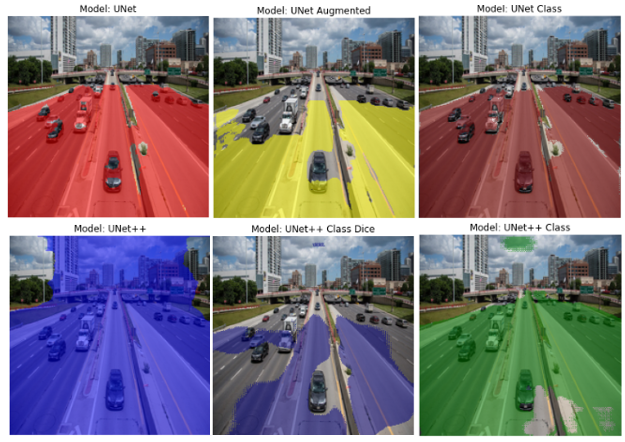
\includegraphics[width=1\linewidth]{dron_view.png} % 그림 파일 이름과 너비 설정
    \caption{드론 카메라 위치에서 촬영된 사진에 대한 모델 비교 결과} % 캡션 추가
    \label{fig:road_detection} % 레이블 설정 (참조용)
\end{figure}

자율주행 데이터에서 도로 결함을 검출하는 각 모델의 성능을 평가하고, 저공 비행 드론에 적용했을 때의 성능 변화를 분석한다. 실험 결과는 다음과 같다.
\begin{figure}[!h]
    \centering
    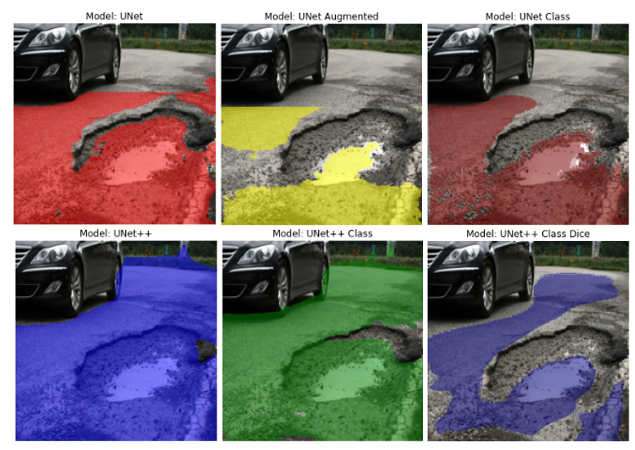
\includegraphics[width=1\linewidth]{lane_crack.png} % 그림 파일 이름과 너비 설정
    \caption{도로 결함에 대한 각 모델 비교 결과} % 캡션 추가
    \label{fig:crack_detection} % 레이블 설정 (참조용)
\end{figure}

\subsection{이진 분류 세그멘테이션 결과}
U-Net 모델은 구조가 단순하여 연산 속도가 빠르고, 다양한 조명 조건에서도 안정적인 성능을 보였다. U-Net++ 모델은 Dice 손실을 사용하여 불균형 데이터 상황에서 더욱 우수한 결함 탐지 성능을 나타냈다.

\subsection{다중 클래스 세그멘테이션 결과}
다중 클래스 세그멘테이션에서는 U-Net++ 모델이 U-Net 모델보다 높은 성능을 보였다. 특히 Dice 손실을 추가하여 불균형 클래스에 대한 성능이 개선되었으며, Road IoU 메트릭을 통해 세분화된 결함 탐지 성능이 측정되었다.

\subsection{손실 함수와 메트릭의 영향}
Dice 손실을 적용한 U-Net++ 모델에서는 다중 클래스 세그멘테이션 성능이 유의미하게 향상되었으며, Dice 계수와 Road IoU를 동시에 사용하는 것이 정확도를 높이는 데 기여하였다.


\section{Conclusion}

본 연구에서는 자율주행 데이터를 사용한 도로 결함 탐지에서 이진 분류와 다중 분류 세그멘테이션 접근을 비교하였다. U-Net++ 모델은 다중 클래스 세그멘테이션에서 더 높은 성능을 보여주었으며, Dice 손실을 추가하여 불균형 클래스 문제를 개선하였다. 이 연구는 자율주행 데이터가 저공 비행 드론의 인프라 점검에도 유용하게 활용될 수 있음을 시사하며, 향후 경량화된 모델과 최적화된 손실 함수를 통해 실시간 응용 가능성을 높이고자 한다.



\bibliographystyle{IEEEtran}
\bibliography{reference}

\end{document}

